\documentclass[conference]{IEEEtran}

\usepackage[T1]{fontenc}
\usepackage[utf8]{inputenc}
\usepackage{cite}
\usepackage{amsmath,amssymb,amsfonts}
\usepackage{siunitx}
\usepackage{booktabs}
\usepackage{array}
\usepackage{multirow}
\usepackage{graphicx}
\usepackage{xcolor}
\usepackage{listings}
\usepackage{tikz}
\usepackage{pgfplots}
\usepackage{hyperref}
\usepackage{enumitem}
\usepackage{float}
\usetikzlibrary{arrows.meta,positioning,shapes.geometric,fit,calc}
\pgfplotsset{compat=1.18}

\hypersetup{hidelinks}
\sisetup{detect-all}

\lstdefinestyle{shellstyle}{
  basicstyle=\ttfamily\footnotesize,
  frame=single,
  breaklines=true,
  columns=fullflexible,
  keepspaces=true
}

\title{Yet Another Audio analyzeR (YAAR):\\
A Real-Time FFT-Based Audio Measurement Tool for Distortion, Noise, and Power Analysis}

\author{\IEEEauthorblockN{George Biro}
\IEEEauthorblockA{Independent Developer\\
GPLv3-or-later\\
Email: george.biro@gmail.com}}

\begin{document}
\maketitle

\begin{abstract}
This paper presents Yet Another Audio analyzeR (YAAR), a lightweight command-line and interactive plotting tool for real-time audio analysis, together with a separate signal generator utility for deterministic test signal synthesis. The analyzer combines time-domain monitoring, FFT-based spectral estimation, rolling magnitude averaging, automatic tone detection, and measurement of total harmonic distortion (THD), total harmonic distortion plus noise (THD+N), intermodulation distortion (IMD), signal-to-noise ratio (SNR), signal-to-noise-and-distortion ratio (SINAD), effective number of bits (ENOB), and electrical output metrics such as $V_{\mathrm{RMS}}$ and $P_{\mathrm{RMS}}$.

YAAR supports both live acquisition from an audio backend and an internal simulation mode, while the accompanying generator produces phase-continuous single-tone and two-tone excitation signals for controlled measurements. The two programs can be used independently or combined to form a complete measurement chain, enabling real-time analysis, repeatable simulation, and end-to-end validation of audio systems.

The implementation was validated on a \mbox{MacBook Air M4} using a \mbox{Cosmos ADC (E1DA)}, a \mbox{UNI-T UTG932E} signal generator, and a \mbox{FiiO BR3} Bluetooth device used as a DAC.

This document serves as a professional user and technical manual, describing the operating principles, command-line interfaces, measurement workflow, configuration parameters, and practical usage recommendations.
\end{abstract}

\begin{IEEEkeywords}
audio measurement, FFT, THD, THD+N, IMD, SNR, SINAD, ENOB, spectrum analysis, Python
\end{IEEEkeywords}

\section{Introduction}
Audio test workflows often require a compact toolset that can both generate controlled excitation signals and analyze responses in real time, without the overhead of a full laboratory software suite. YAAR addresses the analysis side of this requirement with a lightweight Python implementation centered on FFT-based processing and a clear operational model.

In addition to the analyzer, the project includes a separate signal generator utility, enabling deterministic single-tone and two-tone stimulus generation. The two programs can be used independently or combined to form a complete measurement chain, supporting both purely simulated scenarios and end-to-end hardware validation.

The analyzer supports either a physical input stream or an internal simulation path, making it suitable for both bench measurements and algorithm development, while the external generator enables validation of real signal paths including DACs, amplifiers, and ADCs.

The software is designed around the following goals:
\begin{enumerate}[leftmargin=*,nosep]
    \item real-time visualization of the waveform and spectrum,
    \item robust spectral metric extraction under single-tone and two-tone conditions,
    \item deterministic signal generation for repeatable test scenarios,
    \item simple command-line configuration,
    \item CSV and plot export for reproducible reporting.
\end{enumerate}

\section{System Overview}
At runtime, YAAR repeatedly acquires or synthesizes a measurement block, applies a selected window function, computes a real FFT, updates a rolling spectrum average, detects one or two dominant tones, builds masks for the fundamental and distortion components, and derives scalar metrics for display and export.

\begin{figure}[t]
\centering
\resizebox{\columnwidth}{!}{%
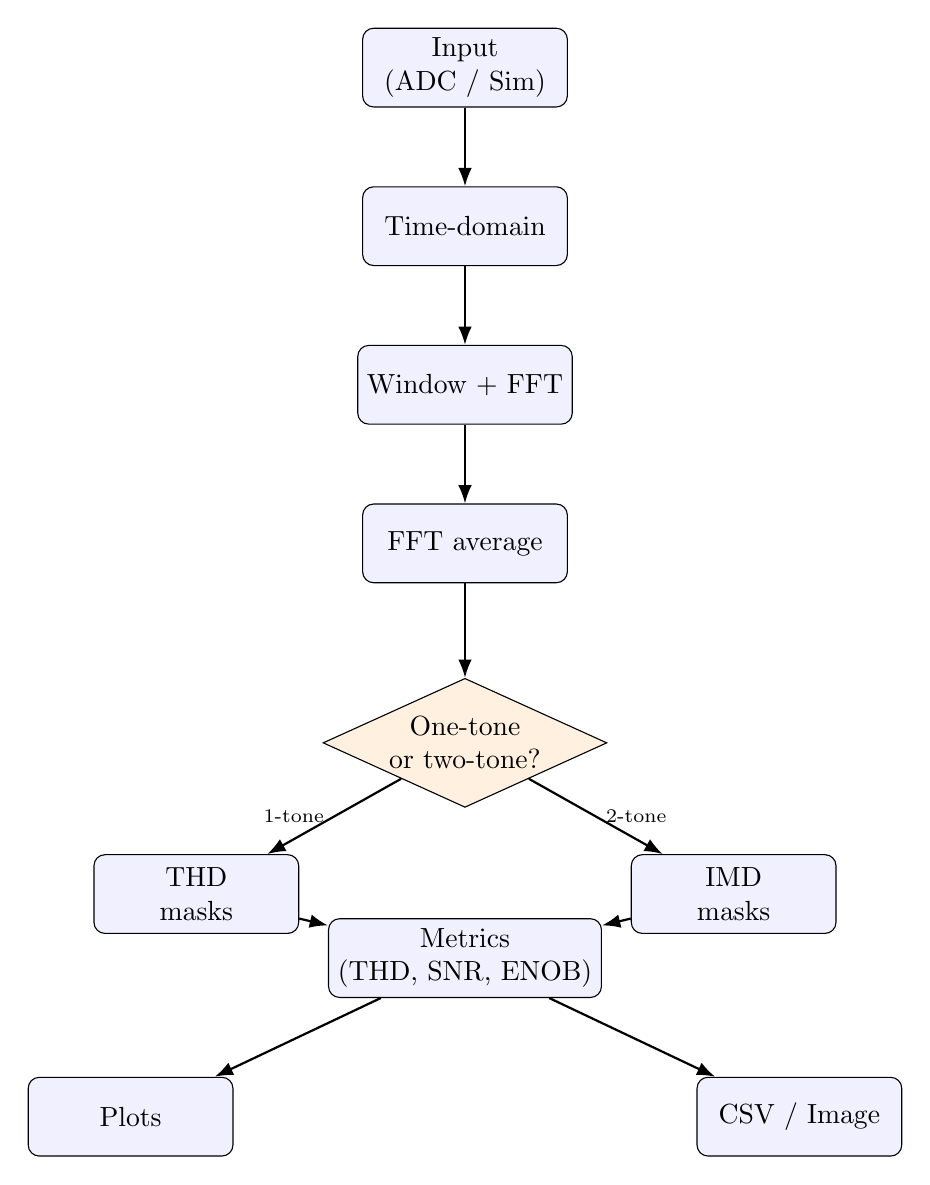
\begin{tikzpicture}[
    transform shape,
    node distance=10mm and 10mm,
    block/.style={
        draw,
        rounded corners,
        align=center,
        minimum width=2.6cm,
        minimum height=1cm,
        fill=blue!6
    },
    decision/.style={
        draw,
        diamond,
        aspect=2.2,
        align=center,
        fill=orange!12,
        inner sep=1pt
    },
    line/.style={-Latex, thick}
]

% ---- Top pipeline ----
\node[block] (input) {Input\\(ADC / Sim)};
\node[block, below=of input] (td) {Time-domain};
\node[block, below=of td] (fft) {Window + FFT};
\node[block, below=of fft] (avg) {FFT average};

% ---- Decision BELOW avg (correct logic) ----
\node[decision, below=12mm of avg] (mode) {One-tone\\or two-tone?};

% ---- Branches BELOW decision ----
\node[block, below left=10mm and 12mm of mode] (single) {THD\\masks};
\node[block, below right=10mm and 12mm of mode] (double) {IMD\\masks};

% ---- Merge BELOW ----
\node[block, below=14mm of mode] (metrics) {Metrics\\(THD, SNR, ENOB)};

% ---- Outputs ----
\node[block, below left=10mm and 12mm of metrics] (plot) {Plots};
\node[block, below right=10mm and 12mm of metrics] (export) {CSV / Image};

% ---- Connections ----
\draw[line] (input) -- (td);
\draw[line] (td) -- (fft);
\draw[line] (fft) -- (avg);

\draw[line] (avg) -- (mode);

\draw[line] (mode) -- node[left, font=\scriptsize] {1-tone} (single);
\draw[line] (mode) -- node[right, font=\scriptsize] {2-tone} (double);

\draw[line] (single) -- (metrics);
\draw[line] (double) -- (metrics);

\draw[line] (metrics) -- (plot);
\draw[line] (metrics) -- (export);

\end{tikzpicture}%
}
\caption{High-level YAAR processing flow.}
\label{fig:overview}
\end{figure}

\section{Software Architecture}
The main program logic is organized around a continuous measurement loop. Several helper functions and lightweight classes encapsulate reusable behavior:
\begin{itemize}[leftmargin=*,nosep]
    \item \textbf{\texttt{simulate\_signal}} generates one-tone or two-tone synthetic signals with optional additive noise and distortion.
    \item \textbf{\texttt{RollingFFTAverage}} smooths frame-to-frame FFT magnitude variation by averaging power spectra over a sliding window.
    \item \textbf{\texttt{WRef}} constructs a spectral kernel corresponding to a windowed sinusoid and shifts it to expected tone bins.
    \item \textbf{Peak detection and mask builders} determine whether the measurement is best interpreted as THD or IMD.
    \item \textbf{Metric functions} convert partitioned spectral powers into engineering quantities such as THD, THD+N, SNR, and ENOB.
\end{itemize}

\begin{figure}[t]
\centering
\resizebox{\columnwidth}{!}{%
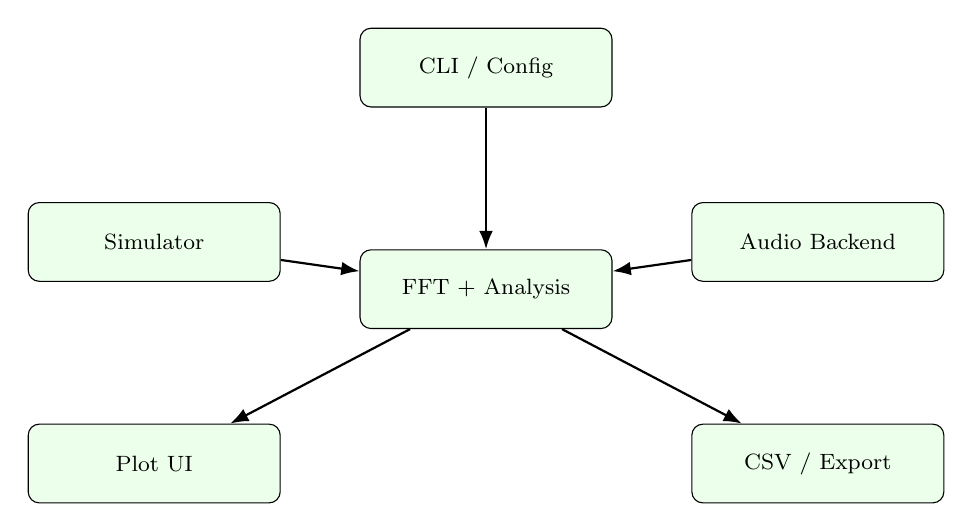
\begin{tikzpicture}[
    transform shape,
    font=\footnotesize,
    node distance=12mm,
    box/.style={
        draw,
        rounded corners,
        minimum width=3.2cm,
        minimum height=1cm,
        align=center,
        fill=green!8
    },
    line/.style={-Latex, thick}
]

% --- Left: configuration ---
\node[box] (cfg) {CLI / Config};

% --- Inputs ---
\node[box, below left=12mm and 10mm of cfg] (sim) {Simulator};
\node[box, below right=12mm and 10mm of cfg] (backend) {Audio Backend};

% --- Core ---
\node[box, below=18mm of cfg] (core) {FFT + Analysis};

% --- Outputs ---
\node[box, below left=12mm and 10mm of core] (ui) {Plot UI};
\node[box, below right=12mm and 10mm of core] (out) {CSV / Export};

% --- Connections (NO crossings) ---
\draw[line] (cfg) -- (core);

\draw[line] (sim) -- (core);
\draw[line] (backend) -- (core);

\draw[line] (core) -- (ui);
\draw[line] (core) -- (out);

\end{tikzpicture}%
}
\caption{Functional organization of YAAR.}
\label{fig:architecture}
\end{figure}

\section{Measurement Theory}
\subsection{FFT Magnitude Estimation}
Given a measurement vector $x[n]$ of length $N$ and a window $w[n]$, YAAR computes the real FFT of $x[n]w[n]$. The resulting magnitude spectrum is corrected for window coherent gain and equivalent noise bandwidth (ENBW):
\begin{equation}
|X[k]| = \frac{|\mathrm{RFFT}\{x[n]w[n]\}|}{N\,G_c\,\sqrt{\mathrm{ENBW}}}
\end{equation}
where
\begin{equation}
G_c = \frac{1}{N}\sum_{n=0}^{N-1} w[n]
\end{equation}
and
\begin{equation}
\mathrm{ENBW} = N\frac{\sum_n w[n]^2}{\left(\sum_n w[n]\right)^2}.
\end{equation}

\subsection{Time-Domain Metrics}
From the raw measurement block, the software computes peak-to-peak voltage, RMS voltage, peak power, and RMS power across a user-defined load resistance $R_L$:
\begin{align}
V_{\mathrm{PP}} &= \max(x)-\min(x) \\
V_{\mathrm{RMS}} &= \sqrt{\frac{1}{N}\sum_n x[n]^2} \\
P_{\mathrm{RMS}} &= \frac{V_{\mathrm{RMS}}^2}{R_L}.
\end{align}

\subsection{Distortion and Noise Metrics}
After spectral masks partition the signal into fundamental, distortion, and noise terms with powers $V_{\mathrm{fund}}$, $V_{\mathrm{dist}}$, and $V_{\mathrm{noise}}$, the primary metrics are:
\begin{align}
\mathrm{THD} &= \sqrt{\frac{V_{\mathrm{dist}}}{V_{\mathrm{fund}}}} \\
\mathrm{THD+N} &= \sqrt{\frac{V_{\mathrm{dist}}+V_{\mathrm{noise}}}{V_{\mathrm{fund}}}} \\
\mathrm{SNR} &= 20\log_{10}\left(\sqrt{\frac{V_{\mathrm{fund}}}{V_{\mathrm{noise}}}}\right) \\
\mathrm{SINAD} &= 20\log_{10}\left(\sqrt{\frac{V_{\mathrm{fund}}}{V_{\mathrm{dist}}+V_{\mathrm{noise}}}}\right) \\
\mathrm{ENOB} &= \frac{\mathrm{SINAD}-1.76}{6.02}.
\end{align}

In two-tone mode, the same computational structure is used, but the distortion mask targets selected intermodulation products rather than harmonic bins.

\section{Tone Detection and Operating Modes}
YAAR automatically switches between single-tone and two-tone operation. It searches for the two strongest frequency bins inside the active analysis band, enforces a minimum frequency separation, and requires the second tone to remain within a user-configurable relative level threshold.

\begin{figure}[t]
\centering
\resizebox{0.9\columnwidth}{!}{%
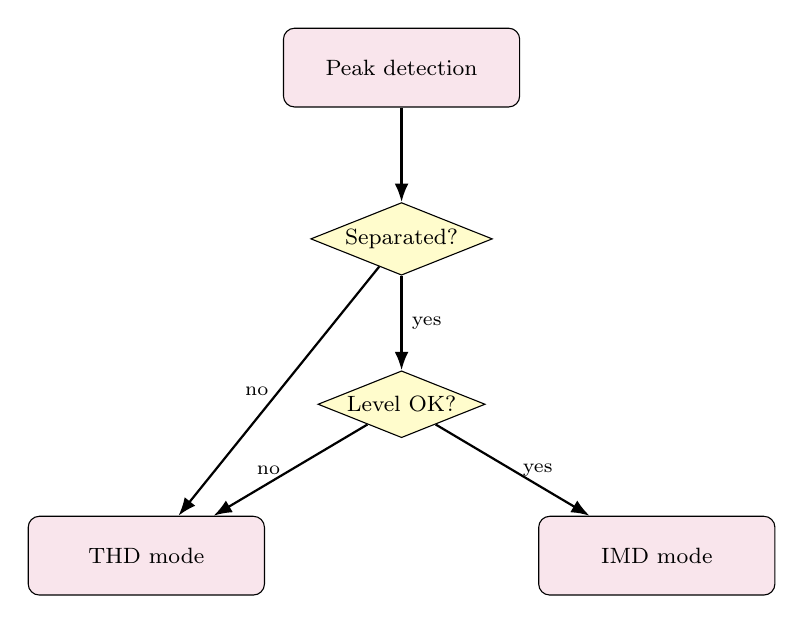
\begin{tikzpicture}[
    transform shape,
    node distance=12mm,
    font=\footnotesize,
    block/.style={
        draw,
        rounded corners,
        align=center,
        minimum width=3cm,
        minimum height=1cm,
        fill=purple!10
    },
    decision/.style={
        draw,
        diamond,
        aspect=2.5,
        align=center,
        fill=yellow!20,
        inner sep=1pt
    },
    line/.style={-Latex, thick}
]

% --- Top ---
\node[block] (search) {Peak detection};

% --- Decisions ---
\node[decision, below=of search] (sep) {Separated?};
\node[decision, below=of sep] (lvl) {Level OK?};

% --- Outputs ---
\node[block, below left=12mm and 12mm of lvl] (thd) {THD mode};
\node[block, below right=12mm and 12mm of lvl] (imd) {IMD mode};

% --- Connections ---
\draw[line] (search) -- (sep);

\draw[line] (sep) -- node[right, font=\scriptsize]{yes} (lvl);
\draw[line] (sep) -- node[left, font=\scriptsize]{no} (thd);

\draw[line] (lvl) -- node[left, font=\scriptsize]{no} (thd);
\draw[line] (lvl) -- node[right, font=\scriptsize]{yes} (imd);

\end{tikzpicture}%
}
\caption{Automatic selection between THD and IMD modes.}
\label{fig:mode}
\end{figure}

\subsection{Single-Tone Mode}
In single-tone mode, the dominant peak is treated as the carrier. A shifted reference kernel estimates the spectral footprint of the windowed sinusoid, and harmonics up to the limit set by \texttt{--thd} are included in the distortion mask.

\subsection{Two-Tone Mode}
In two-tone mode, YAAR builds masks for both fundamentals and a selected set of intermodulation products based on combinations of the two detected tones. The implemented products correspond to common low-order IMD terms derived from $f_1$ and $f_2$.

\section{User Interface}
The display contains three logical regions:
\begin{enumerate}[leftmargin=*,nosep]
    \item a time-domain plot showing the waveform within the selected time span,
    \item a logarithmic frequency-domain plot normalized to the current spectral maximum, and
    \item a status block containing frequency, distortion, noise, ENOB, voltage, power, and reference frequency indicators.
\end{enumerate}

In single-tone mode, spectral annotations label harmonic numbers. In two-tone mode, the principal tones are labeled \texttt{F1} and \texttt{F2}. The display updates continuously until the measurement duration expires, the plot window is closed, or the user interrupts execution.

\section{Command-Line Interface}
Table~\ref{tab:cli} summarizes the public command-line arguments.

\begin{table*}[t]
\centering
\caption{YAAR command-line options.}
\label{tab:cli}
\begin{tabular}{>{\ttfamily}p{2.7cm} p{8.8cm} p{2.0cm}}
\toprule
Option & Meaning & Default \\
\midrule
--list & List available sound devices and exit. & false \\
--freq & Sampling rate in hertz. & 192000 \\
--dev & Audio device index for live capture. & 4 \\
--chsel & Zero-based selected channel. & 1 \\
--chnum & Number of audio channels to open. & 2 \\
--chunk & Requested FFT size; rounded to nearest power of two internally. & 65536 \\
--adcrng & ADC full-scale voltage range. & 100.0 \\
--vrange & Display voltage range for the time plot, shown as $\pm$ value. & 40.0 \\
--frange & Upper frequency shown in the spectrum plot. Lower bound is fixed at \SI{10}{Hz}. & 70000.0 \\
--trange & Time span displayed in milliseconds. & 100.0 \\
--wrange & Lower dB bound of the spectral plot. Upper bound is \SI{0}{dB}. & -150.0 \\
--rload & Load resistance used for power calculations. & 8.0 \\
--thd & Number of harmonic orders included in THD mode. & 7 \\
--duration & Maximum runtime in seconds. & 240 \\
--plot & Base path for exported plot image. Saved after signal stabilization. & empty \\
--csv & CSV path for appending measurement records. & empty \\
--window & Window function: bartlett, blackman, hamming, hanning/hann, rect. & hanning \\
--simfreq & Fundamental frequency for simulation mode. If positive, live input is bypassed. & 0.0 \\
--simnoise & Simulated white-noise amplitude in dB relative scale. & -160.0 \\
--flttsh & Threshold used to convert reference kernels into binary masks, in dB. & 120.0 \\
--cftsh & Center-frequency threshold parameter stored in configuration. & 0.25 \\
--twotone-rel-db & Maximum allowed level drop for the second tone to enter IMD mode. & 16.0 \\
--peak-sep-hz & Minimum spacing between detected fundamentals for IMD mode. & 20.0 \\
--simfreq2 & Second simulated tone frequency. & 0.0 \\
--simamp2 & Relative amplitude of the second simulated tone. & 1.0 \\
--simhmncs & Simulated distortion strength for harmonics or IMD products. & 0.0 \\
\bottomrule
\end{tabular}
\end{table*}

\section{Practical Usage}
\subsection{Listing Devices}
Before using live capture, identify the desired audio input device:
\begin{lstlisting}[style=shellstyle]
python yaar.py --list
\end{lstlisting}

\subsection{Basic Live Measurement}
A typical real-input run at \SI{192}{kHz} with an \SI{8}{\ohm} load is:
\begin{lstlisting}[style=shellstyle]
python yaar.py --freq 192000 --chunk 65536 --rload 8
\end{lstlisting}

\subsection{Single-Tone Simulation}
To validate the software path without audio hardware:
\begin{lstlisting}[style=shellstyle]
python yaar.py --simfreq 1000
\end{lstlisting}

\subsection{Noisy and Distorted Simulation}
\begin{lstlisting}[style=shellstyle]
python yaar.py --simfreq 1000 --simnoise -90 --simhmncs 0.01
\end{lstlisting}

\subsection{Two-Tone IMD Measurement}
\begin{lstlisting}[style=shellstyle]
python yaar.py --simfreq 1000 --simfreq2 1200 --simamp2 1.0
\end{lstlisting}

\subsection{CSV Logging and Plot Export}
\begin{lstlisting}[style=shellstyle]
python yaar.py --simfreq 1000 --csv results.csv --plot spectrum.png
\end{lstlisting}
When the detected carrier remains stable for the required number of iterations, YAAR appends a CSV record and optionally saves plot images.

If plot export is enabled (via \texttt{--plot}), the analyzer generates one output image per detected frequency configuration. The file names follow the pattern:
\begin{center}
\texttt{<base>\_<freq1>hz\_<freq2>hz.png}
\end{center}
where \texttt{<base>} is the user-provided path and \texttt{freq1}, \texttt{freq2} are the detected fundamental frequencies. In single-tone mode, the second frequency is set to zero.

This behavior allows straightforward automated analysis and batch processing, as multiple measurement conditions produce uniquely identifiable output files.

\section{CSV Output Format}
When a CSV path is provided and the file does not yet exist, YAAR writes a header row with the following fields:
\begin{center}
\footnotesize
\texttt{Mode, F1\_hz, F2\_hz, THDN\_dB, THDN\_pct, THD\_dB, THD\_pct,}\newline
\texttt{IMDN\_dB, IMDN\_pct, IMD\_dB, IMD\_pct, SINAD\_db, SNR\_dB, ENOB,}\newline
\texttt{Vrms, Prms, FFT size, Sample Rate}
\end{center}

The \texttt{Mode} field is set to \texttt{THD} or \texttt{IMD}. In single-tone operation, the second-frequency field is zero.

\section{Simulation Model}
The simulator can synthesize the following scenarios:
\begin{itemize}[leftmargin=*,nosep]
    \item a single sinusoid with random phase,
    \item an optional second sinusoid with independent random phase,
    \item additive white Gaussian noise, and
    \item either harmonic distortion or selected IMD products scaled to a target relative amplitude.
\end{itemize}

When only one simulated tone is present, the distortion generator creates harmonic terms from the second through the user-selected harmonic count. When two tones are present, the same parameter instead scales a predefined set of low-order intermodulation products.

\section{Window Functions}
YAAR supports Bartlett, Blackman, Hamming, Hann/Hanning, and rectangular windows. The selected window influences leakage, amplitude accuracy, and noise bandwidth. The default Hann window is a balanced choice for general-purpose measurement because it provides good sidelobe suppression while preserving straightforward interpretation.

\section{Recommendations for Accurate Measurements}
\begin{itemize}[leftmargin=*,nosep]
    \item Use a sufficiently large FFT size, such as 65536 or larger when latency permits.
    \item Keep the input signal below clipping limits in both the analog front end and the digital capture path.
    \item For best frequency estimation and leakage control, choose stable sources and appropriate windowing.
    \item Verify channel selection and device index before assuming a measurement issue.
    \item In two-tone testing, ensure the tones are separated by more than \texttt{--peak-sep-hz} and that the second tone remains within the configured relative level threshold.
\end{itemize}

\section{Limitations and Implementation Notes}
The following implementation details are important to understand:
\begin{itemize}[leftmargin=*,nosep]
    \item The requested FFT size is rounded to the nearest power of two.
    \item The displayed frequency range always starts at \SI{10}{Hz}, regardless of the upper bound selected with \texttt{--frange}.
    \item Spectrum values are displayed relative to the current maximum in the visible band rather than as absolute calibrated dBV or dBFS.
    \item CSV writing and plot saving occur only after a stability counter reaches its threshold.
    \item The audio interface itself is delegated to the external \texttt{audio\_backend} module.
\end{itemize}

A small code-level observation is worth noting for users interpreting exported CSV data: the CSV header places \texttt{SINAD\_db} before \texttt{SNR\_dB}, while the write function currently writes the values in the order \texttt{snr\_db} followed by \texttt{sinad\_db}. If strict column alignment matters for downstream analysis, verify this mapping in your post-processing pipeline.

\section{Signal Generator Utility}

\subsection{Overview}
In addition to the YAAR analyzer, the project provides a separate command-line program (\texttt{gen.py}) for real-time audio signal generation. The generator is an independent tool and can be used either together with YAAR or as a standalone excitation source for external measurement setups.

Its primary purpose is to provide controlled and repeatable test signals for:
\begin{itemize}[leftmargin=*,nosep]
    \item distortion and noise measurements,
    \item intermodulation testing,
    \item system validation of ADC/DAC chains, and
    \item calibration and verification tasks.
\end{itemize}

\subsection{Relationship to YAAR}
The generator and analyzer are intentionally decoupled:
\begin{itemize}[leftmargin=*,nosep]
    \item \textbf{YAAR (\texttt{yaar.py})} performs acquisition, FFT analysis, and metric extraction.
    \item \textbf{Generator (\texttt{gen.py})} produces deterministic excitation signals.
\end{itemize}

They may be used:
\begin{itemize}[leftmargin=*,nosep]
    \item independently, or
    \item together as a measurement pair (e.g., generator output looped into analyzer input).
\end{itemize}

YAAR also includes an internal simulation mode; however, the external generator enables testing of full hardware signal paths.

\subsection{Design Principles}
The generator uses a \textit{phase accumulator} architecture to ensure:
\begin{itemize}[leftmargin=*,nosep]
    \item frequency accuracy independent of buffer size,
    \item phase continuity across blocks,
    \item absence of discontinuities or clicks, and
    \item deterministic long-duration behavior.
\end{itemize}

\subsection{Signal Model}
The generated waveform consists of one or two sinusoidal components:
\begin{equation}
x[n] = A_1 \sin(\phi_1[n]) + A_2 \sin(\phi_2[n])
\end{equation}

with phase evolution:
\begin{equation}
\phi_k[n+1] = \phi_k[n] + \frac{2\pi f_k}{f_s}, \quad k \in \{1,2\}.
\end{equation}

The second tone is optional and defined via an amplitude ratio:
\begin{equation}
A_2 = \frac{A_1}{r}
\end{equation}

The output is scaled by a global level parameter:
\begin{equation}
y[n] = \alpha \cdot x[n], \quad \alpha \in [0,1].
\end{equation}

\subsection{Implementation}
The generator is implemented as a \texttt{SineGenerator} class maintaining:
\begin{itemize}[leftmargin=*,nosep]
    \item phase accumulators,
    \item phase increments derived from frequency and sample rate,
    \item amplitude scaling for multi-tone operation.
\end{itemize}

Audio output is produced as a continuous stream of 32-bit floating-point samples.

\subsection{Command-Line Interface}
\begin{table}[t]
\centering
\caption{Signal generator command-line options.}
\label{tab:gen_cli}
\begin{tabular}{>{\ttfamily}p{2.6cm} p{4.8cm}}
\toprule
Option & Description \\
\midrule
--list & List available output devices \\
--dev & Output device index \\
--rate & Sampling rate (Hz) \\
--chunk & Block size (samples) \\
--freq & Primary tone frequency (Hz) \\
--freq2 & Secondary tone frequency (Hz) \\
--ratio & Amplitude ratio A/B \\
--level & Output amplitude scaling (0..1) \\
--time & Run time in seconds (0 = continuous) \\
\bottomrule
\end{tabular}
\end{table}

The \texttt{--time} parameter enables bounded-duration execution, which is particularly useful for automated testing and scripting. When specified, the generator runs for the given number of seconds and then exits cleanly, allowing integration into batch pipelines or regression test frameworks. A value of \texttt{0} results in continuous operation until interrupted.

\subsection{Example Usage}
\begin{lstlisting}[style=shellstyle]
# List output devices
python gen.py --list

# Single-tone signal
python gen.py --dev 2 --freq 1000

# Two-tone IMD test
python gen.py --dev 2 --freq 1000 --freq2 1200 --ratio 1

# Limited duration test
python gen.py --dev 2 --freq 1000 --time 10
\end{lstlisting}

\subsection{Limitations}
\begin{itemize}[leftmargin=*,nosep]
    \item Single-channel output
    \item No built-in dithering or noise shaping
    \item Performance limited by Python execution at very high rates
\end{itemize}

\subsection{Summary}
The generator complements YAAR by providing a stable and controllable excitation source. While YAAR supports internal simulation, the external generator enables full end-to-end testing of real-world signal chains.

\section{Requirements and Execution}

\subsection{Software Requirements}
Both YAAR (\texttt{yaar.py}) and the signal generator (\texttt{gen.py}) are implemented in Python and require:

\begin{itemize}[leftmargin=*,nosep]
    \item Python 3.9 or newer
    \item \texttt{numpy} for numerical processing
    \item \texttt{matplotlib} for visualization (YAAR)
    \item an audio I/O library (e.g.\ \texttt{pyaudio} or equivalent backend)
\end{itemize}

\subsection{Hardware Requirements}
\begin{itemize}[leftmargin=*,nosep]
    \item For analysis: a compatible audio input device
    \item For signal generation: a compatible audio output device
    \item For loopback testing: physical or virtual connection between output and input
\end{itemize}

\subsection{Program Execution}
Both tools are executed independently from the command line:

\begin{lstlisting}[style=shellstyle]
# Run analyzer
python yaar.py [options]

# Run generator
python gen.py [options]
\end{lstlisting}

\subsection{Combined Operation}
A typical measurement setup uses both tools together:
\begin{itemize}[leftmargin=*,nosep]
    \item \texttt{gen.py} produces the excitation signal
    \item the signal is routed (physically or virtually) to the input
    \item \texttt{yaar.py} performs spectral analysis and metric extraction
\end{itemize}

\section{Example Measurement Result}

\subsection{Single tone THD example}

Figure~\ref{fig:simtest_1k} shows a representative measurement obtained using the internal simulation mode with a non-integer tone frequency, added harmonic distortion, and elevated noise floor.

\begin{lstlisting}[style=shellstyle]
python yaar.py --simfreq 987.3 --simhmncs 0.01 --simnoise -60
\end{lstlisting}

The resulting spectrum illustrates the detected fundamental, harmonic components, and noise distribution as processed by the FFT-based analysis pipeline.

\begin{figure}[H]
\centering
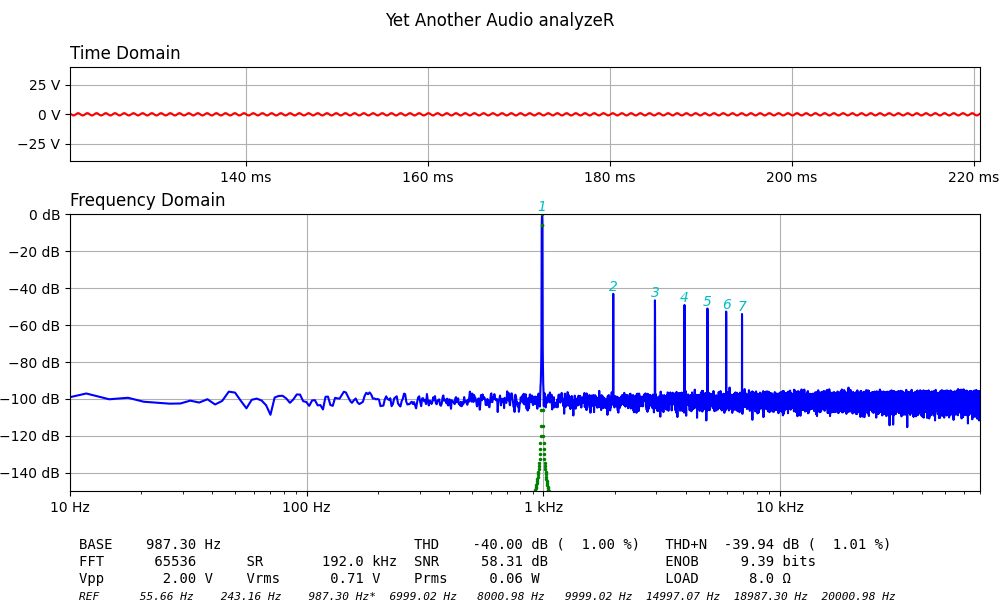
\includegraphics[width=0.9\columnwidth]{simtest_987Hz_0Hz.png}
\caption{Example spectrum for simulated input at \SI{987.3}{Hz} with added distortion and noise.}
\label{fig:simtest_1k}
\end{figure}

No direct coupling between the programs is required.

\subsection{Two-Tone IMD Example}

Figure~\ref{fig:simtest_7khz_60hz} shows a simulated two-tone measurement illustrating intermodulation distortion behavior. Two tones at low and high frequency are combined with added distortion and noise.

\begin{lstlisting}[style=shellstyle]
python yaar.py --simfreq 55.66 --simfreq2 6999.02 --simhmncs 0.01 --simnoise -40
\end{lstlisting}

The resulting spectrum demonstrates automatic transition into IMD mode, with identification of the two fundamental tones and the appearance of intermodulation products generated by the nonlinear distortion model.

\begin{figure}[H]
\centering
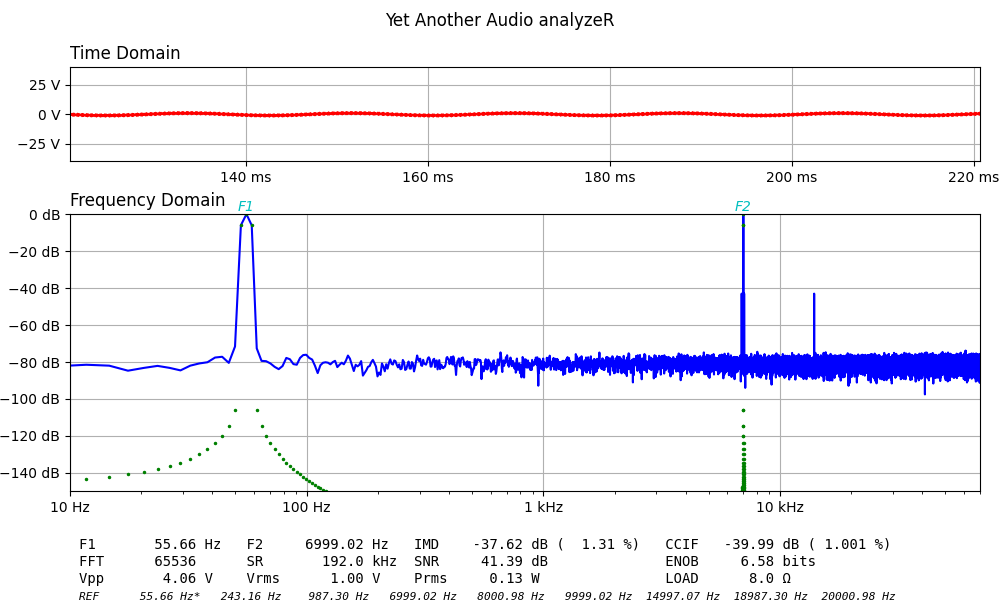
\includegraphics[width=0.9\columnwidth]{simtest_56Hz_6999Hz.png}
\caption{Two-tone IMD example with tones at \SI{55.66}{Hz} and \SI{6999.02}{Hz}, including distortion and noise.}
\label{fig:simtest_7khz_60hz}
\end{figure}

\subsection{Hardware Single-Tone Measurement Example}

Figure~\ref{fig:hwtest_987hz} shows a measurement performed using a UNI-T UTG932E signal generator, configured at \SI{987.3}{Hz}, and connected to a COSMOS E1DA ADC.

This setup represents a real hardware measurement chain, where the generator provides a stable excitation signal and the ADC captures the response for FFT-based analysis in YAAR. The resulting spectrum demonstrates practical system performance, including noise floor and distortion components introduced by the physical signal path.

\begin{figure}[H]
\centering
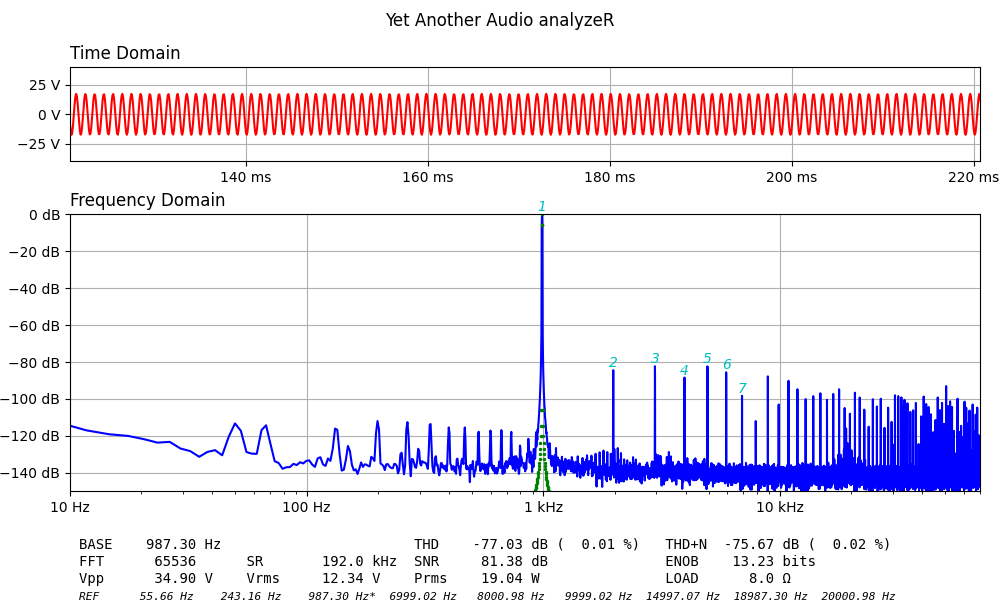
\includegraphics[width=0.9\columnwidth]{unit_utg932e_987Hz_0Hz.png}
\caption{Hardware measurement using a UNI-T UTG932E signal generator at \SI{987.3}{Hz} and a COSMOS E1DA ADC.}
\label{fig:hwtest_987hz}
\end{figure}

\subsection{Hardware Two-Tone IMD (CCIF) Measurement Example}

Figure~\ref{fig:hwtest_ccif} shows a two-tone measurement using a FiiO BR13 connected to a COSMOS E1DA ADC. The excitation signal was generated using:

\begin{lstlisting}[style=shellstyle]
python gen.py --dev 0 --freq 243.16 --freq2 6999.02
\end{lstlisting}

This configuration produces a CCIF-style intermodulation test, where two widely spaced tones are used to evaluate nonlinear behavior. The resulting spectrum allows observation of intermodulation distortion (IMD) products, including sum and difference components, as well as higher-order mixing artifacts.

Both IMD and CCIF-related distortion components can be identified and evaluated directly from the spectral output.

\begin{figure}[H]
\centering
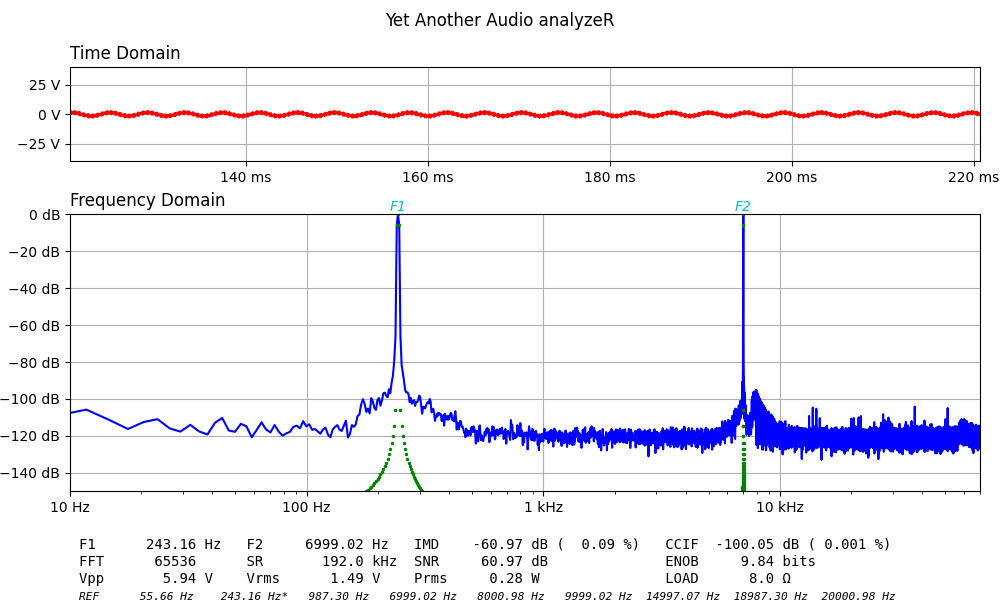
\includegraphics[width=0.9\columnwidth]{fiio3br_243Hz_6999Hz.png}
\caption{Two-tone IMD (CCIF) measurement using FiiO BR13 and COSMOS E1DA ADC with tones at \SI{243.16}{Hz} and \SI{6999.02}{Hz}.}
\label{fig:hwtest_ccif}
\end{figure}

\section{Troubleshooting}
\subsection{No Input or Empty Display}
Check the selected device index with \texttt{--list}, verify the correct channel number, and confirm that the chosen device supports the requested sample rate.

\subsection{Unexpected Noise Floor}
Increase the FFT size, confirm proper grounding and shielding in the analog setup, and inspect whether the selected window is appropriate for the stimulus.

\subsection{Two-Tone Mode Does Not Trigger}
Reduce \texttt{--twotone-rel-db} only if the second tone is intentionally weak, and ensure that the tone separation exceeds \texttt{--peak-sep-hz}.

\subsection{Power Values Seem Incorrect}
Verify the configured load resistance \texttt{--rload} and confirm that the input voltage scaling in the backend is calibrated correctly.

\section{Conclusion}
YAAR is a compact but capable audio measurement tool that integrates real-time visualization with practically relevant spectral metrics. Its combination of a live backend, a synthetic signal path, automatic operating-mode selection, rolling FFT averaging, and export support makes it useful for rapid evaluation of amplifiers, ADCs, DACs, and other audio signal chains. The architecture is intentionally simple and transparent, which also makes the program a suitable starting point for custom extensions.

\section*{Appendix: Quick Command Reference}
\begin{lstlisting}[style=shellstyle]
# List audio devices
python yaar.py --list

# Live measurement
python yaar.py --freq 192000 --dev 4 --chsel 1 --chnum 2

# Single-tone simulation
python yaar.py --simfreq 1000

# THD-style simulation with noise and harmonics
python yaar.py --simfreq 1000 --simnoise -100 --simhmncs 0.02

# Two-tone IMD simulation
python yaar.py --simfreq 19000 --simfreq2 20000 --simamp2 1.0

# Export CSV and plot
python yaar.py --simfreq 1000 --csv out.csv --plot out.png
\end{lstlisting}

\end{document}
